% -*- mode: noweb; noweb-default-code-mode: R-mode; -*-


\documentclass{article}

\usepackage{arxiv}

\usepackage[utf8]{inputenc} % allow utf-8 input
\usepackage[T1]{fontenc}    % use 8-bit T1 fonts
\usepackage{hyperref}       % hyperlinks
\usepackage{url}            % simple URL typesetting
\usepackage{booktabs}       % professional-quality tables
\usepackage{amsfonts}       % blackboard math symbols
\usepackage{amssymb}        % needed for \leqslant
\usepackage{amsmath}        % needed for cases
\usepackage{nicefrac}       % compact symbols for 1/2, etc.
\usepackage{microtype}      % microtypography
\usepackage{lipsum}		% Can be removed after putting your text content
\usepackage{graphicx}
\usepackage{natbib}
\usepackage{doi}



\title{Clifford algebra in R}

%\date{September 9, 1985}	% Here you can change the date presented in the paper title
%\date{} 					% Or removing it

\author{ \href{https://orcid.org/0000-0001-5982-0415}{\includegraphics[width=0.03\textwidth]{orcid.pdf}\hspace{1mm}Robin K. S.~Hankin}\thanks{\href{https://academics.aut.ac.nz/robin.hankin}{work};  
\href{https://www.youtube.com/watch?v=JzCX3FqDIOc&list=PL9_n3Tqzq9iWtgD8POJFdnVUCZ_zw6OiB&ab_channel=TrinTragulaGeneralRelativity}{play}} \\
 Auckland University of Technology\\
	\texttt{hankin.robin@gmail.com} \\
}

% Uncomment to remove the date
%\date{}

% Uncomment to override  the `A preprint' in the header
%\renewcommand{\headeright}{Technical Report}
%\renewcommand{\undertitle}{Technical Report}
\renewcommand{\shorttitle}{The \textit{clifford} package}

%%% Add PDF metadata to help others organize their library
%%% Once the PDF is generated, you can check the metadata with
%%% $ pdfinfo template.pdf
\hypersetup{
pdftitle={Clifford algebra in R},
pdfsubject={q-bio.NC, q-bio.QM},
pdfauthor={Robin K. S.~Hankin},
pdfkeywords={Clifford algebra}
}

\usepackage{Sweave}
\begin{document}
\maketitle

\begin{abstract}
Here I present the {\tt clifford} package for working with Clifford
algebras in the R programming language.  The algebra is described and
package idiom is given.
\end{abstract}


% keywords can be removed
\keywords{Clifford algebra}



\hfill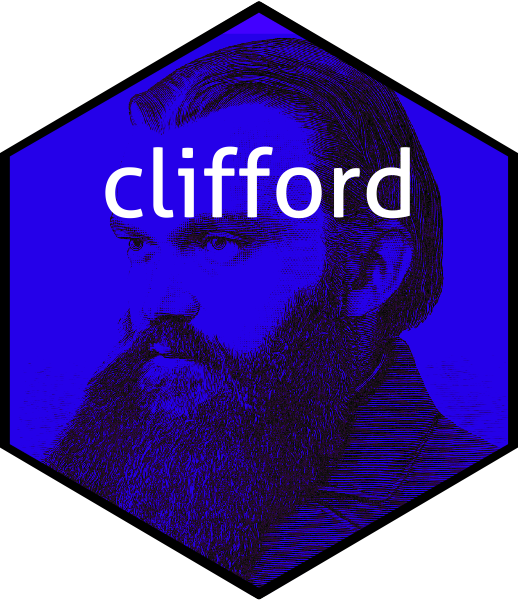
\includegraphics[width=1in]{clifford.png}

\section{Introduction}

Clifford algebras are interesting and instructive mathematical
objects.  The class has a rich structure that has varied applications
to physics.

\subsection{Existing work}

Computational support for working with the Clifford algebras is part
of a number of algebra systems including Sage~\citep{sagemath2019} and
\textit{sympy}~\citep{sympy2017}.  Here I introduce the
\textit{clifford} package, which provides R-centric functionality for
Clifford algebras.  Notation follows~\cite{snygg2010}.


\newcommand{\ei}[1]{\ensuremath{{\bf e}_{#1}}}
\newcommand{\bx}{\ensuremath{{\bf x}}}
\newcommand{\by}{\ensuremath{{\bf y}}}

Considering a vector space of dimension 3, and given a basis
$\ei{1},\ei{2},\ei{3}$, we can consider linear combinations such as

\begin{eqnarray}
\bx = x^1\ei{1} + x^2\ei{2} + x^3\ei{3}\nonumber\\
\by = y^1\ei{1} + y^2\ei{2} + y^3\ei{3}.
\end{eqnarray} 

A Clifford algebra includes a formal product on such sums, defined using the
relations

\begin{eqnarray}\label{square}
\left(\ei{1}\right)^2=
\left(\ei{2}\right)^2=
\left(\ei{3}\right)^2=1\\
\ei{2}\ei{3} + \ei{3}\ei{2} = \label{sumprod}
\ei{1}\ei{3} + \ei{3}\ei{1} = 
\ei{2}\ei{1} + \ei{1}\ei{2} = 0
\end{eqnarray}

This gives:
  
\begin{eqnarray}
\bx\by &=&
\left(x^1\ei{1} + x^2\ei{2} + x^3\ei{3}\right)
\left(y^1\ei{1} + y^2\ei{2} + y^3\ei{3}\right)\nonumber\\
&=& \left(x^1y^1+x^2y^2+x^3y^3\right) +\nonumber\\&&
       \left(x^2y^3-x^3y^2\right)\ei{2}\ei{3} + 
       \left(x^3y^1-x^1y^3\right)\ei{1}\ei{3} + 
       \left(x^1y^2-x^2y^1\right)\ei{1}\ei{2}
\end{eqnarray}
  
Multiplication is associative by design.  \citeauthor{snygg2010} goes
on to consider the algebra spanned by products of
$\ei{1},\ei{2},\ei{3}$ and shows that this is an eight dimensional
space spanned by

\begin{equation}
\left\{
1,\ei{1},\ei{2},\ei{3},\ei{12},\ei{31},\ei{12},\ei{123}
\right\}
\end{equation}

where $\ei{12}=\ei{1}\ei{2}$ and so on.  Thus a general element of
this space would be

\begin{equation}
a^0+
a^1\ei{1} + a^2\ei{2} + a^3\ei{3} +
a^{12}\ei{12} + a^{31}\ei{31} + a^{23}\ei{23} +
a^{123}\ei{123}
\end{equation}

(here the $a$'s are real).  That the space is closed under
multiplication follows from equations~\ref{square} and~\ref{sumprod};
thus, for example,

\begin{equation}
  \ei{1}\ei{3}\ei{1}\ei{2}=
 -\ei{1}\ei{1}\ei{3}\ei{2}=
 -\ei{3}\ei{2}=
  \ei{2}\ei{3}=\ei{23}.
  \end{equation}

(observe how associativity is assumed).

\subsection{Generalization to arbitrary dimensions}

Generalization to higher dimensional vector spaces is easy.  Suppose
we consider a $n$-dimensional vector space spanned by
$\ei{1},\ldots,\ei{n}$.  Then an arbitrary vector in this space will
be $a^1\ei{1}+\cdots+a^n\ei{n}$.  The associated Clifford algebra will
be of dimension $2^n$, spanned by elements like
$\ei{1}\ei{3}\ei{5}=\ei{135}$ and
$\ei{1}\ei{2}\ei{3}\ei{5}=\ei{1235}$.  The defining relations would be

\begin{equation}\label{posdefcliff}
\ei{i}\ei{j}+\ei{j}\ei{i}=2n_{ij}
\end{equation}
where  
\begin{equation}\label{posdefcliff2}
  n_{ij} = \begin{cases}
    1, & i=j\\
    0 &i\neq j
  \end{cases}
\end{equation}



\subsection{Clifford algebra in a pseudo-Euclidean space}

Equations~\ref{posdefcliff} and~\ref{posdefcliff2} defined a
positive-definite inner product on the vector space spanned
by~$\ei{1},\ei{2},\ei{3}$.  This is readily generalized to allow a
more general inner product.  Conventionally we define

\begin{equation}\label{gencliff1}
\ei{i}\ei{j}+\ei{j}\ei{i}=2n_{ij}
\end{equation}
where  
\begin{equation}\label{gencliff2}
  n_{ij} = \begin{cases}
    1, & i=j=1,\ldots,p\\
    -1, & i=j=p+1,\ldots,n\\
    0, &i\neq j
  \end{cases}
\end{equation}

for $1\leqslant p\leqslant n$; usually we also specify $p+q=n$ and
write $\mathbb{R}_{p,q}$ for the $p+q$-dimensional vector space with
inner product given by equation~\ref{gencliff1}.  The Clifford algebra
${\mathcal C}_{p,q}$ (other notations include $Cl(p,q)$) is then the
algebra formed by $\mathbb{R}_{p,q}$ together with formal products of
basis vectors.


Note carefully that the diagonal matrix of the inner product specified
above conventionally has the the positive elements first, followed by
the negative elements.  But in relativity, the metric tensor $\eta$ is
usually written with the negative elements first followed by the
positive elements;

\begin{equation}\eta=
  \begin{bmatrix}
    -1&0&0&0\\
    0&1&0&0\\
    0&0&1&0\\
    0&0&0&1\\
  \end{bmatrix}
\end{equation}


\subsection{Wedge product of the exterior algebra is a special case
  of the geometric product}

If we specify that the quadratic form is identically zero then
equation \ref{gencliff1} becomes

\begin{equation}\label{specwedge}
\ei{i}\ei{j}+\ei{j}\ei{i}=0,\qquad 1\leqslant i,j\leqslant p
\end{equation}

which implies that $\ei{i}\ei{i}=0$.  Geometric products become wedge
products (although linearity means that we may add terms of different
grades, unlike conventional Grassman algebra).

\section{The package in use}

Suppose we want to work with arbitrary Clifford object
$1+2\ei{1}+3\ei{2}+4\ei{2}\ei{3}$.  In R idiom this would be

\begin{Schunk}
\begin{Sinput}
> (x <- clifford(list(numeric(0),1,2,2:3),1:4))
\end{Sinput}
\begin{Soutput}
Element of a Clifford algebra, equal to
+ 1 + 2e_1 + 3e_2 + 4e_23
\end{Soutput}
\end{Schunk}

Function {\tt clifford()} takes a list of terms and a vector of
coefficients.  Addition and subtraction work as expected:

\begin{Schunk}
\begin{Sinput}
> y <- clifford(list(1),2)
> x-y
\end{Sinput}
\begin{Soutput}
Element of a Clifford algebra, equal to
+ 1 + 3e_2 + 4e_23
\end{Soutput}
\end{Schunk}

In the above, see how the $\ei{1}$ term has vanished.  We can
multiply Clifford elements using natural R idiom:

\begin{Schunk}
\begin{Sinput}
> x*x
\end{Sinput}
\begin{Soutput}
Element of a Clifford algebra, equal to
- 2 + 4e_1 + 6e_2 + 8e_23 + 16e_123
\end{Soutput}
\end{Schunk}

(Multiplication that Snygg denotes by juxtaposition is here indicated
with a {\tt *}).  We can consider arbitrarily high dimensional data:

\begin{Schunk}
\begin{Sinput}
> (z <- as.1vector(1:7))
\end{Sinput}
\begin{Soutput}
Element of a Clifford algebra, equal to
+ 1e_1 + 2e_2 + 3e_3 + 4e_4 + 5e_5 + 6e_6 + 7e_7
\end{Soutput}
\begin{Sinput}
> z*x
\end{Sinput}
\begin{Soutput}
Element of a Clifford algebra, equal to
+ 8 + 1e_1 - 10e_2 - 1e_12 + 11e_3 - 6e_13 - 9e_23 + 4e_123 + 4e_4 - 8e_14 -
12e_24 + 16e_234 + 5e_5 - 10e_15 - 15e_25 + 20e_235 + 6e_6 - 12e_16 - 18e_26 +
24e_236 + 7e_7 - 14e_17 - 21e_27 + 28e_237
\end{Soutput}
\end{Schunk}

In the above, we coerce a vector to a Clifford 1-vector.  The package
includes many functions to generate Clifford objects:

\begin{Schunk}
\begin{Sinput}
> rcliff()
\end{Sinput}
\begin{Soutput}
Element of a Clifford algebra, equal to
+ 4 - 2e_4 + 4e_24 + 5e_1234 - 1e_15 + 1e_35 - 3e_45 + 2e_256
\end{Soutput}
\end{Schunk}

The defaults for {\tt rcliff()} specify that the object is a sum of
grade-4 terms but this can be altered:

\begin{Schunk}
\begin{Sinput}
> (x <- rcliff(d=7,g=5,include.fewer=TRUE))
\end{Sinput}
\begin{Soutput}
Element of a Clifford algebra, equal to
+ 4 + 1e_4 - 3e_6 + 3e_12356 + 2e_7 - 1e_23467 + 4e_567 + 5e_3567
\end{Soutput}
\begin{Sinput}
> grades(x)
\end{Sinput}
\begin{Soutput}
A disord object with hash 2d7dd83887de1b90a47d1fef514bb2f733b30b83 and elements
[1] 0 1 1 5 1 5 3 4
(in some order)
\end{Soutput}
\end{Schunk}


\section{Pseudo-Euclidean spaces}

The signature of the metric may be altered.  Starting with the
Euclidean case we have:
    
\begin{Schunk}
\begin{Sinput}
> e1 <- e(1)
> e2 <- e(2)
> e1*e1
\end{Sinput}
\begin{Soutput}
Element of a Clifford algebra, equal to
scalar ( 1 )
\end{Soutput}
\begin{Sinput}
> e2*e2
\end{Sinput}
\begin{Soutput}
Element of a Clifford algebra, equal to
scalar ( 1 )
\end{Soutput}
\end{Schunk}

(function {\tt e(i)} returns $\ei{i}$).  However, if we wish to
consider $n=\begin{bmatrix}1&0\\0&-1\end{bmatrix}$, the package idiom
is to use the {\tt signature()} function:

\begin{Schunk}
\begin{Sinput}
> signature(1,1)  # signature +-
> e1*e1 # as before, returns +1
\end{Sinput}
\begin{Soutput}
Element of a Clifford algebra, equal to
scalar ( 1 )
\end{Soutput}
\begin{Sinput}
> e2*e2 # should return -1
\end{Sinput}
\begin{Soutput}
Element of a Clifford algebra, equal to
scalar ( -1 )
\end{Soutput}
\end{Schunk}

Suppose we wish to use a signature $+++-$, corresponding to the
Minkowski metric in special relativity; this would be indicated in
package idiom by {\tt signature(3,1)}.  Note that the clifford objects
themselves do not store the signature; it is used only by the product
operation {\tt *}.

\begin{Schunk}
\begin{Sinput}
> x <- rcliff(d=4,g=3,include.fewer=TRUE)
> y <- rcliff(d=4,g=3,include.fewer=TRUE)
\end{Sinput}
\end{Schunk}

Then we may multiply these two clifford objects using either the
default positive-definite inner product, or the Minkowski metric:

\begin{Schunk}
\begin{Sinput}
> x*y
\end{Sinput}
\begin{Soutput}
Element of a Clifford algebra, equal to
+ 12 + 12e_1 - 6e_2 + 6e_12 + 7e_3 - 7e_13 + 21e_23 + 13e_123 + 9e_24 + 9e_124
+ 2e_34 + 8e_134 + 19e_234 - 11e_1234
\end{Soutput}
\begin{Sinput}
> signature(3,1)  # switch to signature +++-
> x*y
\end{Sinput}
\begin{Soutput}
Element of a Clifford algebra, equal to
+ 30 + 16e_1 + 2e_12 + 5e_3 - 11e_13 + 21e_23 + 16e_123 - 1e_4 - 18e_14 +
14e_24 + 17e_124 - 2e_34 + 19e_234 - 11e_1234
\end{Soutput}
\end{Schunk}

In the above, see how the products are different using the two inner
products.  

\section{Grassman algebra}

A Grassman algebra corresponds to a Clifford algebra with identically
zero inner product.  Package idiom is to use a zero signature:

\begin{Schunk}
\begin{Sinput}
> signature(0,0)  # specify null inner product
\end{Sinput}
\end{Schunk}
\begin{Schunk}
\begin{Sinput}
> is.zero(e(5)^2)     # should be TRUE
\end{Sinput}
\begin{Soutput}
[1] TRUE
\end{Soutput}
\end{Schunk}

This is a somewhat clunky way of reproducing the functionality of the
{\tt stokes} package.  If we have

\begin{Schunk}
\begin{Sinput}
> x <- clifford(list(1:3, c(2,3,7)), coeffs=3:4)
> y <- clifford(list(1:3, c(1,4,5), c(4,5,6)), coeffs=1:3)
> x %^% y
\end{Sinput}
\begin{Soutput}
Element of a Clifford algebra, equal to
+ 9e_123456 - 8e_123457 - 12e_234567
\end{Soutput}
\end{Schunk}

then the {\tt stokes} idiom for this would be:

\begin{Schunk}
\begin{Sinput}
> (x <- as.kform(rbind(1:3,c(2,3,7)),3:4))
\end{Sinput}
\begin{Soutput}
           val
 2 3 7  =    4
 1 2 3  =    3
\end{Soutput}
\begin{Sinput}
> (y <- as.kform(rbind(1:3,c(1,4,5),4:6),1:3))
\end{Sinput}
\begin{Soutput}
           val
 1 2 3  =    1
 1 4 5  =    2
 4 5 6  =    3
\end{Soutput}
\begin{Sinput}
> x %^% y
\end{Sinput}
\begin{Soutput}
                 val
 1 2 3 4 5 6  =    9
 2 3 4 5 6 7  =  -12
 1 2 3 4 5 7  =   -8
\end{Soutput}
\end{Schunk}


\section{Positive-definite inner product}

Function {\tt signature()} takes an infinite argument to make the
inner product positive-definite:

\begin{Schunk}
\begin{Sinput}
> signature(Inf)
\end{Sinput}
\end{Schunk}

(internally the package sets the signature to
{\tt .Machine\$integer.max}, a near-infinite integer).  With this,
$\ei{i}\ei{i}=+1$ for any $i$:

\begin{Schunk}
\begin{Sinput}
> e(53)^2
\end{Sinput}
\begin{Soutput}
Element of a Clifford algebra, equal to
scalar ( 1 )
\end{Soutput}
\end{Schunk}


\section{Left and right contractions}

\cite{dorst2002} defines the left contraction $A\rfloor B$ and right
contraction $A\lfloor B$ (\cite{chisholm2012} calls these left and
right inner products) as follows:

\begin{eqnarray}
\displaystyle A\rfloor B = \sum_{r,s}\left\langle\left\langle
A\right\rangle_r\left\langle B\right\rangle_s\right\rangle_{s-r}\\
\displaystyle A\lfloor B = \sum_{r,s}\left\langle\left\langle
A\right\rangle_r\left\langle B\right\rangle_s\right\rangle_{r-s}
\end{eqnarray}


Package idiom for these would be {\tt A\%\_|\%B} and {\tt A\%|\_\%B}
---or {\tt lefttick(A,B)} and {\tt righttick(A,B)}---respectively.
Thus:

\begin{Schunk}
\begin{Sinput}
> (A <- rcliff())
\end{Sinput}
\begin{Soutput}
Element of a Clifford algebra, equal to
+ 4 + 2e_2 - 2e_34 + 3e_35 + 5e_235 - 1e_145 + 1e_46 + 4e_156
\end{Soutput}
\begin{Sinput}
> (B <- rcliff())
\end{Sinput}
\begin{Soutput}
Element of a Clifford algebra, equal to
+ 3 - 3e_1 - 1e_13 + 2e_4 + 1e_34 + 3e_135 + 4e_345
\end{Soutput}
\begin{Sinput}
> A %_|% B
\end{Sinput}
\begin{Soutput}
Element of a Clifford algebra, equal to
+ 14 - 21e_1 - 4e_13 + 20e_4 + 4e_34 + 8e_5 + 12e_135 + 16e_345
\end{Soutput}
\begin{Sinput}
> A %|_% B
\end{Sinput}
\begin{Soutput}
Element of a Clifford algebra, equal to
+ 14 + 6e_2 - 4e_3 - 6e_34 + 2e_15 + 9e_35 + 15e_235 + 3e_45 - 3e_145 - 2e_6 +
3e_46 - 12e_56 + 12e_156
\end{Soutput}
\end{Schunk}

One thing to be wary of is the order of operations.  Thus
$\ei{2}\rfloor\ei{12}=-\ei{1}$ (in a positive-definite space) but

\begin{Schunk}
\begin{Sinput}
> e(2) %_|% e(1)*e(2)
\end{Sinput}
\begin{Soutput}
Element of a Clifford algebra, equal to
the zero clifford element (0)
\end{Soutput}
\end{Schunk}

because this is parsed as $(\ei{2}\rfloor\ei{1})\ei{2}=0\ei{2}=0$.  To
evaluate this as intended we need to include brackets:

\begin{Schunk}
\begin{Sinput}
> e(2) %_|% (e(1)*e(2))
\end{Sinput}
\begin{Soutput}
Element of a Clifford algebra, equal to
- 1e_1
\end{Soutput}
\end{Schunk}

although in this case it might be preferable to create the terms directly:

\begin{Schunk}
\begin{Sinput}
> e(2) %_|% e(1:2)
\end{Sinput}
\begin{Soutput}
Element of a Clifford algebra, equal to
- 1e_1
\end{Soutput}
\end{Schunk}


\subsection{Numerical verification of left and right inner product identities}

Chisholm gives a number of identities for these products including

\begin{eqnarray}
  A\rfloor(B\lfloor C) &=& (A\rfloor B)\lfloor C\\
  A\rfloor(B\rfloor C) &=& (A\wedge B)\rfloor C\\
  A\lfloor(B\wedge  C) &=& (A\lfloor B)\lfloor C
\end{eqnarray}

In package idiom:

\begin{Schunk}
\begin{Sinput}
> A <- rcliff();  B <- rcliff();  C <- rcliff()
> A %_|% (B %|_% C) == (A %_|% B) %|_% C
\end{Sinput}
\begin{Soutput}
[1] TRUE
\end{Soutput}
\begin{Sinput}
> A %_|% (B %_|% C) == (A %^%  B) %_|% C
\end{Sinput}
\begin{Soutput}
[1] TRUE
\end{Soutput}
\begin{Sinput}
> A %|_% (B %^%  C) == (A %|_% B) %|_% C
\end{Sinput}
\begin{Soutput}
[1] TRUE
\end{Soutput}
\end{Schunk}
\section{Higher dimensional spaces}

\cite{ablamowicz2012} consider high-dimensional Clifford algebras and
consider the following two elements of the 1024-dimensional Clifford
algebra which we may treat as ${\mathcal C}_{7,3}$ spanned by
$\ei{1},\ldots,\ei{10}$ and perform a calculation which I reproduce
below (although \citeauthor{ablamowicz2012} exploited Bott
periodicity, a feature not considered here).

Firstly we change the default print method slightly:

\begin{Schunk}
\begin{Sinput}
> options("basissep" = ",")
\end{Sinput}
\end{Schunk}

(this separates the subscripts of the basis vectors with a comma,
which is useful for clarity if $n>9$).  We then define clifford
elements $x,y$:

\begin{Schunk}
\begin{Sinput}
> (x <- clifford(list(1:3,c(1,5,7,8,10)),c(4,-10)) + 2)
\end{Sinput}
\begin{Soutput}
Element of a Clifford algebra, equal to
+ 2 + 4e_1,2,3 - 10e_1,5,7,8,10
\end{Soutput}
\begin{Sinput}
> (y <- clifford(list(c(1,2,3,7),c(1,5,6,8),c(1,4,6,7)),c(4,1,-3)) - 1)
\end{Sinput}
\begin{Soutput}
Element of a Clifford algebra, equal to
- 1 + 4e_1,2,3,7 - 3e_1,4,6,7 + 1e_1,5,6,8
\end{Soutput}
\end{Schunk}

Their geometric product is given in the package as

\begin{Schunk}
\begin{Sinput}
> signature(7)
> x*y
\end{Sinput}
\begin{Soutput}
Element of a Clifford algebra, equal to
- 2 - 4e_1,2,3 - 16e_7 + 8e_1,2,3,7 - 6e_1,4,6,7 - 12e_2,3,4,6,7 + 2e_1,5,6,8 +
4e_2,3,5,6,8 - 40e_2,3,5,8,10 - 30e_4,5,6,8,10 + 10e_1,5,7,8,10
\end{Soutput}
\end{Schunk}

in agreement with \cite{ablamowicz2012}, although the terms appear in
a different order.

\section{Conclusions and further work}

The {\tt clifford} package furnishes a consistent and documented suite
of reasonably efficient {\tt R}-centric functionality.  Further
work might include closer integration with the {\tt stokes}
package~\citep{hankin2019}.


 
\bibliographystyle{apalike}
% -*- mode: noweb; noweb-default-code-mode: R-mode; -*-


\documentclass{article}

\usepackage{arxiv}

\usepackage[utf8]{inputenc} % allow utf-8 input
\usepackage[T1]{fontenc}    % use 8-bit T1 fonts
\usepackage{hyperref}       % hyperlinks
\usepackage{url}            % simple URL typesetting
\usepackage{booktabs}       % professional-quality tables
\usepackage{amsfonts}       % blackboard math symbols
\usepackage{amssymb}        % needed for \leqslant
\usepackage{amsmath}        % needed for cases
\usepackage{nicefrac}       % compact symbols for 1/2, etc.
\usepackage{microtype}      % microtypography
\usepackage{lipsum}		% Can be removed after putting your text content
\usepackage{graphicx}
\usepackage{natbib}
\usepackage{doi}



\title{Clifford algebra in R}

%\date{September 9, 1985}	% Here you can change the date presented in the paper title
%\date{} 					% Or removing it

\author{ \href{https://orcid.org/0000-0001-5982-0415}{\includegraphics[width=0.03\textwidth]{orcid.pdf}\hspace{1mm}Robin K. S.~Hankin}\thanks{\href{https://academics.aut.ac.nz/robin.hankin}{work};  
\href{https://www.youtube.com/watch?v=JzCX3FqDIOc&list=PL9_n3Tqzq9iWtgD8POJFdnVUCZ_zw6OiB&ab_channel=TrinTragulaGeneralRelativity}{play}} \\
 Auckland University of Technology\\
	\texttt{hankin.robin@gmail.com} \\
}

% Uncomment to remove the date
%\date{}

% Uncomment to override  the `A preprint' in the header
%\renewcommand{\headeright}{Technical Report}
%\renewcommand{\undertitle}{Technical Report}
\renewcommand{\shorttitle}{The \textit{clifford} package}

%%% Add PDF metadata to help others organize their library
%%% Once the PDF is generated, you can check the metadata with
%%% $ pdfinfo template.pdf
\hypersetup{
pdftitle={Clifford algebra in R},
pdfsubject={q-bio.NC, q-bio.QM},
pdfauthor={Robin K. S.~Hankin},
pdfkeywords={Clifford algebra}
}

\usepackage{Sweave}
\begin{document}
\maketitle

\begin{abstract}
Here I present the {\tt clifford} package for working with Clifford
algebras in the R programming language.  The algebra is described and
package idiom is given.
\end{abstract}


% keywords can be removed
\keywords{Clifford algebra}



\hfill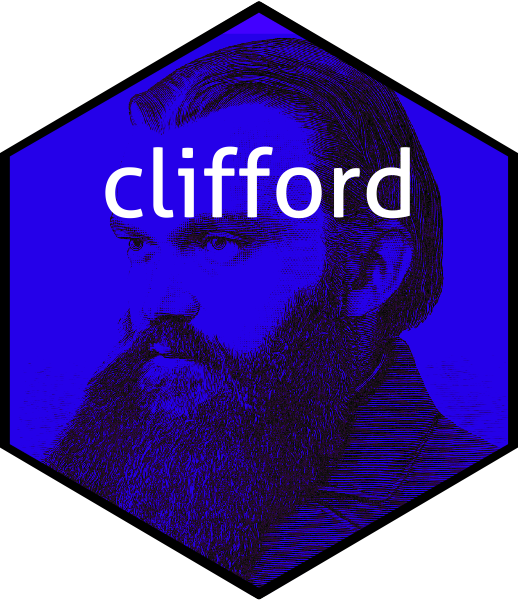
\includegraphics[width=1in]{clifford.png}

\section{Introduction}

Clifford algebras are interesting and instructive mathematical
objects.  The class has a rich structure that has varied applications
to physics.

\subsection{Existing work}

Computational support for working with the Clifford algebras is part
of a number of algebra systems including Sage~\citep{sagemath2019} and
\textit{sympy}~\citep{sympy2017}.  Here I introduce the
\textit{clifford} package, which provides R-centric functionality for
Clifford algebras.  Notation follows~\cite{snygg2010}.


\newcommand{\ei}[1]{\ensuremath{{\bf e}_{#1}}}
\newcommand{\bx}{\ensuremath{{\bf x}}}
\newcommand{\by}{\ensuremath{{\bf y}}}

Considering a vector space of dimension 3, and given a basis
$\ei{1},\ei{2},\ei{3}$, we can consider linear combinations such as

\begin{eqnarray}
\bx = x^1\ei{1} + x^2\ei{2} + x^3\ei{3}\nonumber\\
\by = y^1\ei{1} + y^2\ei{2} + y^3\ei{3}.
\end{eqnarray} 

A Clifford algebra includes a formal product on such sums, defined using the
relations

\begin{eqnarray}\label{square}
\left(\ei{1}\right)^2=
\left(\ei{2}\right)^2=
\left(\ei{3}\right)^2=1\\
\ei{2}\ei{3} + \ei{3}\ei{2} = \label{sumprod}
\ei{1}\ei{3} + \ei{3}\ei{1} = 
\ei{2}\ei{1} + \ei{1}\ei{2} = 0
\end{eqnarray}

This gives:
  
\begin{eqnarray}
\bx\by &=&
\left(x^1\ei{1} + x^2\ei{2} + x^3\ei{3}\right)
\left(y^1\ei{1} + y^2\ei{2} + y^3\ei{3}\right)\nonumber\\
&=& \left(x^1y^1+x^2y^2+x^3y^3\right) +\nonumber\\&&
       \left(x^2y^3-x^3y^2\right)\ei{2}\ei{3} + 
       \left(x^3y^1-x^1y^3\right)\ei{1}\ei{3} + 
       \left(x^1y^2-x^2y^1\right)\ei{1}\ei{2}
\end{eqnarray}
  
Multiplication is associative by design.  \citeauthor{snygg2010} goes
on to consider the algebra spanned by products of
$\ei{1},\ei{2},\ei{3}$ and shows that this is an eight dimensional
space spanned by

\begin{equation}
\left\{
1,\ei{1},\ei{2},\ei{3},\ei{12},\ei{31},\ei{12},\ei{123}
\right\}
\end{equation}

where $\ei{12}=\ei{1}\ei{2}$ and so on.  Thus a general element of
this space would be

\begin{equation}
a^0+
a^1\ei{1} + a^2\ei{2} + a^3\ei{3} +
a^{12}\ei{12} + a^{31}\ei{31} + a^{23}\ei{23} +
a^{123}\ei{123}
\end{equation}

(here the $a$'s are real).  That the space is closed under
multiplication follows from equations~\ref{square} and~\ref{sumprod};
thus, for example,

\begin{equation}
  \ei{1}\ei{3}\ei{1}\ei{2}=
 -\ei{1}\ei{1}\ei{3}\ei{2}=
 -\ei{3}\ei{2}=
  \ei{2}\ei{3}=\ei{23}.
  \end{equation}

(observe how associativity is assumed).

\subsection{Generalization to arbitrary dimensions}

Generalization to higher dimensional vector spaces is easy.  Suppose
we consider a $n$-dimensional vector space spanned by
$\ei{1},\ldots,\ei{n}$.  Then an arbitrary vector in this space will
be $a^1\ei{1}+\cdots+a^n\ei{n}$.  The associated Clifford algebra will
be of dimension $2^n$, spanned by elements like
$\ei{1}\ei{3}\ei{5}=\ei{135}$ and
$\ei{1}\ei{2}\ei{3}\ei{5}=\ei{1235}$.  The defining relations would be

\begin{equation}\label{posdefcliff}
\ei{i}\ei{j}+\ei{j}\ei{i}=2n_{ij}
\end{equation}
where  
\begin{equation}\label{posdefcliff2}
  n_{ij} = \begin{cases}
    1, & i=j\\
    0 &i\neq j
  \end{cases}
\end{equation}



\subsection{Clifford algebra in a pseudo-Euclidean space}

Equations~\ref{posdefcliff} and~\ref{posdefcliff2} defined a
positive-definite inner product on the vector space spanned
by~$\ei{1},\ei{2},\ei{3}$.  This is readily generalized to allow a
more general inner product.  Conventionally we define

\begin{equation}\label{gencliff1}
\ei{i}\ei{j}+\ei{j}\ei{i}=2n_{ij}
\end{equation}
where  
\begin{equation}\label{gencliff2}
  n_{ij} = \begin{cases}
    1, & i=j=1,\ldots,p\\
    -1, & i=j=p+1,\ldots,n\\
    0, &i\neq j
  \end{cases}
\end{equation}

for $1\leqslant p\leqslant n$; usually we also specify $p+q=n$ and
write $\mathbb{R}_{p,q}$ for the $p+q$-dimensional vector space with
inner product given by equation~\ref{gencliff1}.  The Clifford algebra
${\mathcal C}_{p,q}$ (other notations include $Cl(p,q)$) is then the
algebra formed by $\mathbb{R}_{p,q}$ together with formal products of
basis vectors.


Note carefully that the diagonal matrix of the inner product specified
above conventionally has the the positive elements first, followed by
the negative elements.  But in relativity, the metric tensor $\eta$ is
usually written with the negative elements first followed by the
positive elements;

\begin{equation}\eta=
  \begin{bmatrix}
    -1&0&0&0\\
    0&1&0&0\\
    0&0&1&0\\
    0&0&0&1\\
  \end{bmatrix}
\end{equation}


\subsection{Wedge product of the exterior algebra is a special case
  of the geometric product}

If we specify that the quadratic form is identically zero then
equation \ref{gencliff1} becomes

\begin{equation}\label{specwedge}
\ei{i}\ei{j}+\ei{j}\ei{i}=0,\qquad 1\leqslant i,j\leqslant p
\end{equation}

which implies that $\ei{i}\ei{i}=0$.  Geometric products become wedge
products (although linearity means that we may add terms of different
grades, unlike conventional Grassman algebra).

\section{The package in use}

Suppose we want to work with arbitrary Clifford object
$1+2\ei{1}+3\ei{2}+4\ei{2}\ei{3}$.  In R idiom this would be

\begin{Schunk}
\begin{Sinput}
> (x <- clifford(list(numeric(0),1,2,2:3),1:4))
\end{Sinput}
\begin{Soutput}
Element of a Clifford algebra, equal to
+ 1 + 2e_1 + 3e_2 + 4e_23
\end{Soutput}
\end{Schunk}

Function {\tt clifford()} takes a list of terms and a vector of
coefficients.  Addition and subtraction work as expected:

\begin{Schunk}
\begin{Sinput}
> y <- clifford(list(1),2)
> x-y
\end{Sinput}
\begin{Soutput}
Element of a Clifford algebra, equal to
+ 1 + 3e_2 + 4e_23
\end{Soutput}
\end{Schunk}

In the above, see how the $\ei{1}$ term has vanished.  We can
multiply Clifford elements using natural R idiom:

\begin{Schunk}
\begin{Sinput}
> x*x
\end{Sinput}
\begin{Soutput}
Element of a Clifford algebra, equal to
- 2 + 4e_1 + 6e_2 + 8e_23 + 16e_123
\end{Soutput}
\end{Schunk}

(Multiplication that Snygg denotes by juxtaposition is here indicated
with a {\tt *}).  We can consider arbitrarily high dimensional data:

\begin{Schunk}
\begin{Sinput}
> (z <- as.1vector(1:7))
\end{Sinput}
\begin{Soutput}
Element of a Clifford algebra, equal to
+ 1e_1 + 2e_2 + 3e_3 + 4e_4 + 5e_5 + 6e_6 + 7e_7
\end{Soutput}
\begin{Sinput}
> z*x
\end{Sinput}
\begin{Soutput}
Element of a Clifford algebra, equal to
+ 8 + 1e_1 - 10e_2 - 1e_12 + 11e_3 - 6e_13 - 9e_23 + 4e_123 + 4e_4 - 8e_14 -
12e_24 + 16e_234 + 5e_5 - 10e_15 - 15e_25 + 20e_235 + 6e_6 - 12e_16 - 18e_26 +
24e_236 + 7e_7 - 14e_17 - 21e_27 + 28e_237
\end{Soutput}
\end{Schunk}

In the above, we coerce a vector to a Clifford 1-vector.  The package
includes many functions to generate Clifford objects:

\begin{Schunk}
\begin{Sinput}
> rcliff()
\end{Sinput}
\begin{Soutput}
Element of a Clifford algebra, equal to
+ 4 - 2e_4 + 4e_24 + 5e_1234 - 1e_15 + 1e_35 - 3e_45 + 2e_256
\end{Soutput}
\end{Schunk}

The defaults for {\tt rcliff()} specify that the object is a sum of
grade-4 terms but this can be altered:

\begin{Schunk}
\begin{Sinput}
> (x <- rcliff(d=7,g=5,include.fewer=TRUE))
\end{Sinput}
\begin{Soutput}
Element of a Clifford algebra, equal to
+ 4 + 1e_4 - 3e_6 + 3e_12356 + 2e_7 - 1e_23467 + 4e_567 + 5e_3567
\end{Soutput}
\begin{Sinput}
> grades(x)
\end{Sinput}
\begin{Soutput}
A disord object with hash 2d7dd83887de1b90a47d1fef514bb2f733b30b83 and elements
[1] 0 1 1 5 1 5 3 4
(in some order)
\end{Soutput}
\end{Schunk}


\section{Pseudo-Euclidean spaces}

The signature of the metric may be altered.  Starting with the
Euclidean case we have:
    
\begin{Schunk}
\begin{Sinput}
> e1 <- e(1)
> e2 <- e(2)
> e1*e1
\end{Sinput}
\begin{Soutput}
Element of a Clifford algebra, equal to
scalar ( 1 )
\end{Soutput}
\begin{Sinput}
> e2*e2
\end{Sinput}
\begin{Soutput}
Element of a Clifford algebra, equal to
scalar ( 1 )
\end{Soutput}
\end{Schunk}

(function {\tt e(i)} returns $\ei{i}$).  However, if we wish to
consider $n=\begin{bmatrix}1&0\\0&-1\end{bmatrix}$, the package idiom
is to use the {\tt signature()} function:

\begin{Schunk}
\begin{Sinput}
> signature(1,1)  # signature +-
> e1*e1 # as before, returns +1
\end{Sinput}
\begin{Soutput}
Element of a Clifford algebra, equal to
scalar ( 1 )
\end{Soutput}
\begin{Sinput}
> e2*e2 # should return -1
\end{Sinput}
\begin{Soutput}
Element of a Clifford algebra, equal to
scalar ( -1 )
\end{Soutput}
\end{Schunk}

Suppose we wish to use a signature $+++-$, corresponding to the
Minkowski metric in special relativity; this would be indicated in
package idiom by {\tt signature(3,1)}.  Note that the clifford objects
themselves do not store the signature; it is used only by the product
operation {\tt *}.

\begin{Schunk}
\begin{Sinput}
> x <- rcliff(d=4,g=3,include.fewer=TRUE)
> y <- rcliff(d=4,g=3,include.fewer=TRUE)
\end{Sinput}
\end{Schunk}

Then we may multiply these two clifford objects using either the
default positive-definite inner product, or the Minkowski metric:

\begin{Schunk}
\begin{Sinput}
> x*y
\end{Sinput}
\begin{Soutput}
Element of a Clifford algebra, equal to
+ 12 + 12e_1 - 6e_2 + 6e_12 + 7e_3 - 7e_13 + 21e_23 + 13e_123 + 9e_24 + 9e_124
+ 2e_34 + 8e_134 + 19e_234 - 11e_1234
\end{Soutput}
\begin{Sinput}
> signature(3,1)  # switch to signature +++-
> x*y
\end{Sinput}
\begin{Soutput}
Element of a Clifford algebra, equal to
+ 30 + 16e_1 + 2e_12 + 5e_3 - 11e_13 + 21e_23 + 16e_123 - 1e_4 - 18e_14 +
14e_24 + 17e_124 - 2e_34 + 19e_234 - 11e_1234
\end{Soutput}
\end{Schunk}

In the above, see how the products are different using the two inner
products.  

\section{Grassman algebra}

A Grassman algebra corresponds to a Clifford algebra with identically
zero inner product.  Package idiom is to use a zero signature:

\begin{Schunk}
\begin{Sinput}
> signature(0,0)  # specify null inner product
\end{Sinput}
\end{Schunk}
\begin{Schunk}
\begin{Sinput}
> is.zero(e(5)^2)     # should be TRUE
\end{Sinput}
\begin{Soutput}
[1] TRUE
\end{Soutput}
\end{Schunk}

This is a somewhat clunky way of reproducing the functionality of the
{\tt stokes} package.  If we have

\begin{Schunk}
\begin{Sinput}
> x <- clifford(list(1:3, c(2,3,7)), coeffs=3:4)
> y <- clifford(list(1:3, c(1,4,5), c(4,5,6)), coeffs=1:3)
> x %^% y
\end{Sinput}
\begin{Soutput}
Element of a Clifford algebra, equal to
+ 9e_123456 - 8e_123457 - 12e_234567
\end{Soutput}
\end{Schunk}

then the {\tt stokes} idiom for this would be:

\begin{Schunk}
\begin{Sinput}
> (x <- as.kform(rbind(1:3,c(2,3,7)),3:4))
\end{Sinput}
\begin{Soutput}
           val
 2 3 7  =    4
 1 2 3  =    3
\end{Soutput}
\begin{Sinput}
> (y <- as.kform(rbind(1:3,c(1,4,5),4:6),1:3))
\end{Sinput}
\begin{Soutput}
           val
 1 2 3  =    1
 1 4 5  =    2
 4 5 6  =    3
\end{Soutput}
\begin{Sinput}
> x %^% y
\end{Sinput}
\begin{Soutput}
                 val
 1 2 3 4 5 6  =    9
 2 3 4 5 6 7  =  -12
 1 2 3 4 5 7  =   -8
\end{Soutput}
\end{Schunk}


\section{Positive-definite inner product}

Function {\tt signature()} takes an infinite argument to make the
inner product positive-definite:

\begin{Schunk}
\begin{Sinput}
> signature(Inf)
\end{Sinput}
\end{Schunk}

(internally the package sets the signature to
{\tt .Machine\$integer.max}, a near-infinite integer).  With this,
$\ei{i}\ei{i}=+1$ for any $i$:

\begin{Schunk}
\begin{Sinput}
> e(53)^2
\end{Sinput}
\begin{Soutput}
Element of a Clifford algebra, equal to
scalar ( 1 )
\end{Soutput}
\end{Schunk}


\section{Left and right contractions}

\cite{dorst2002} defines the left contraction $A\rfloor B$ and right
contraction $A\lfloor B$ (\cite{chisholm2012} calls these left and
right inner products) as follows:

\begin{eqnarray}
\displaystyle A\rfloor B = \sum_{r,s}\left\langle\left\langle
A\right\rangle_r\left\langle B\right\rangle_s\right\rangle_{s-r}\\
\displaystyle A\lfloor B = \sum_{r,s}\left\langle\left\langle
A\right\rangle_r\left\langle B\right\rangle_s\right\rangle_{r-s}
\end{eqnarray}


Package idiom for these would be {\tt A\%\_|\%B} and {\tt A\%|\_\%B}
---or {\tt lefttick(A,B)} and {\tt righttick(A,B)}---respectively.
Thus:

\begin{Schunk}
\begin{Sinput}
> (A <- rcliff())
\end{Sinput}
\begin{Soutput}
Element of a Clifford algebra, equal to
+ 4 + 2e_2 - 2e_34 + 3e_35 + 5e_235 - 1e_145 + 1e_46 + 4e_156
\end{Soutput}
\begin{Sinput}
> (B <- rcliff())
\end{Sinput}
\begin{Soutput}
Element of a Clifford algebra, equal to
+ 3 - 3e_1 - 1e_13 + 2e_4 + 1e_34 + 3e_135 + 4e_345
\end{Soutput}
\begin{Sinput}
> A %_|% B
\end{Sinput}
\begin{Soutput}
Element of a Clifford algebra, equal to
+ 14 - 21e_1 - 4e_13 + 20e_4 + 4e_34 + 8e_5 + 12e_135 + 16e_345
\end{Soutput}
\begin{Sinput}
> A %|_% B
\end{Sinput}
\begin{Soutput}
Element of a Clifford algebra, equal to
+ 14 + 6e_2 - 4e_3 - 6e_34 + 2e_15 + 9e_35 + 15e_235 + 3e_45 - 3e_145 - 2e_6 +
3e_46 - 12e_56 + 12e_156
\end{Soutput}
\end{Schunk}

One thing to be wary of is the order of operations.  Thus
$\ei{2}\rfloor\ei{12}=-\ei{1}$ (in a positive-definite space) but

\begin{Schunk}
\begin{Sinput}
> e(2) %_|% e(1)*e(2)
\end{Sinput}
\begin{Soutput}
Element of a Clifford algebra, equal to
the zero clifford element (0)
\end{Soutput}
\end{Schunk}

because this is parsed as $(\ei{2}\rfloor\ei{1})\ei{2}=0\ei{2}=0$.  To
evaluate this as intended we need to include brackets:

\begin{Schunk}
\begin{Sinput}
> e(2) %_|% (e(1)*e(2))
\end{Sinput}
\begin{Soutput}
Element of a Clifford algebra, equal to
- 1e_1
\end{Soutput}
\end{Schunk}

although in this case it might be preferable to create the terms directly:

\begin{Schunk}
\begin{Sinput}
> e(2) %_|% e(1:2)
\end{Sinput}
\begin{Soutput}
Element of a Clifford algebra, equal to
- 1e_1
\end{Soutput}
\end{Schunk}


\subsection{Numerical verification of left and right inner product identities}

Chisholm gives a number of identities for these products including

\begin{eqnarray}
  A\rfloor(B\lfloor C) &=& (A\rfloor B)\lfloor C\\
  A\rfloor(B\rfloor C) &=& (A\wedge B)\rfloor C\\
  A\lfloor(B\wedge  C) &=& (A\lfloor B)\lfloor C
\end{eqnarray}

In package idiom:

\begin{Schunk}
\begin{Sinput}
> A <- rcliff();  B <- rcliff();  C <- rcliff()
> A %_|% (B %|_% C) == (A %_|% B) %|_% C
\end{Sinput}
\begin{Soutput}
[1] TRUE
\end{Soutput}
\begin{Sinput}
> A %_|% (B %_|% C) == (A %^%  B) %_|% C
\end{Sinput}
\begin{Soutput}
[1] TRUE
\end{Soutput}
\begin{Sinput}
> A %|_% (B %^%  C) == (A %|_% B) %|_% C
\end{Sinput}
\begin{Soutput}
[1] TRUE
\end{Soutput}
\end{Schunk}
\section{Higher dimensional spaces}

\cite{ablamowicz2012} consider high-dimensional Clifford algebras and
consider the following two elements of the 1024-dimensional Clifford
algebra which we may treat as ${\mathcal C}_{7,3}$ spanned by
$\ei{1},\ldots,\ei{10}$ and perform a calculation which I reproduce
below (although \citeauthor{ablamowicz2012} exploited Bott
periodicity, a feature not considered here).

Firstly we change the default print method slightly:

\begin{Schunk}
\begin{Sinput}
> options("basissep" = ",")
\end{Sinput}
\end{Schunk}

(this separates the subscripts of the basis vectors with a comma,
which is useful for clarity if $n>9$).  We then define clifford
elements $x,y$:

\begin{Schunk}
\begin{Sinput}
> (x <- clifford(list(1:3,c(1,5,7,8,10)),c(4,-10)) + 2)
\end{Sinput}
\begin{Soutput}
Element of a Clifford algebra, equal to
+ 2 + 4e_1,2,3 - 10e_1,5,7,8,10
\end{Soutput}
\begin{Sinput}
> (y <- clifford(list(c(1,2,3,7),c(1,5,6,8),c(1,4,6,7)),c(4,1,-3)) - 1)
\end{Sinput}
\begin{Soutput}
Element of a Clifford algebra, equal to
- 1 + 4e_1,2,3,7 - 3e_1,4,6,7 + 1e_1,5,6,8
\end{Soutput}
\end{Schunk}

Their geometric product is given in the package as

\begin{Schunk}
\begin{Sinput}
> signature(7)
> x*y
\end{Sinput}
\begin{Soutput}
Element of a Clifford algebra, equal to
- 2 - 4e_1,2,3 - 16e_7 + 8e_1,2,3,7 - 6e_1,4,6,7 - 12e_2,3,4,6,7 + 2e_1,5,6,8 +
4e_2,3,5,6,8 - 40e_2,3,5,8,10 - 30e_4,5,6,8,10 + 10e_1,5,7,8,10
\end{Soutput}
\end{Schunk}

in agreement with \cite{ablamowicz2012}, although the terms appear in
a different order.

\section{Conclusions and further work}

The {\tt clifford} package furnishes a consistent and documented suite
of reasonably efficient {\tt R}-centric functionality.  Further
work might include closer integration with the {\tt stokes}
package~\citep{hankin2019}.


 
\bibliographystyle{apalike}
% -*- mode: noweb; noweb-default-code-mode: R-mode; -*-


\documentclass{article}

\usepackage{arxiv}

\usepackage[utf8]{inputenc} % allow utf-8 input
\usepackage[T1]{fontenc}    % use 8-bit T1 fonts
\usepackage{hyperref}       % hyperlinks
\usepackage{url}            % simple URL typesetting
\usepackage{booktabs}       % professional-quality tables
\usepackage{amsfonts}       % blackboard math symbols
\usepackage{amssymb}        % needed for \leqslant
\usepackage{amsmath}        % needed for cases
\usepackage{nicefrac}       % compact symbols for 1/2, etc.
\usepackage{microtype}      % microtypography
\usepackage{lipsum}		% Can be removed after putting your text content
\usepackage{graphicx}
\usepackage{natbib}
\usepackage{doi}



\title{Clifford algebra in R}

%\date{September 9, 1985}	% Here you can change the date presented in the paper title
%\date{} 					% Or removing it

\author{ \href{https://orcid.org/0000-0001-5982-0415}{\includegraphics[width=0.03\textwidth]{orcid.pdf}\hspace{1mm}Robin K. S.~Hankin}\thanks{\href{https://academics.aut.ac.nz/robin.hankin}{work};  
\href{https://www.youtube.com/watch?v=JzCX3FqDIOc&list=PL9_n3Tqzq9iWtgD8POJFdnVUCZ_zw6OiB&ab_channel=TrinTragulaGeneralRelativity}{play}} \\
 Auckland University of Technology\\
	\texttt{hankin.robin@gmail.com} \\
}

% Uncomment to remove the date
%\date{}

% Uncomment to override  the `A preprint' in the header
%\renewcommand{\headeright}{Technical Report}
%\renewcommand{\undertitle}{Technical Report}
\renewcommand{\shorttitle}{The \textit{clifford} package}

%%% Add PDF metadata to help others organize their library
%%% Once the PDF is generated, you can check the metadata with
%%% $ pdfinfo template.pdf
\hypersetup{
pdftitle={Clifford algebra in R},
pdfsubject={q-bio.NC, q-bio.QM},
pdfauthor={Robin K. S.~Hankin},
pdfkeywords={Clifford algebra}
}

\usepackage{Sweave}
\begin{document}
\maketitle

\begin{abstract}
Here I present the {\tt clifford} package for working with Clifford
algebras in the R programming language.  The algebra is described and
package idiom is given.
\end{abstract}


% keywords can be removed
\keywords{Clifford algebra}



\hfill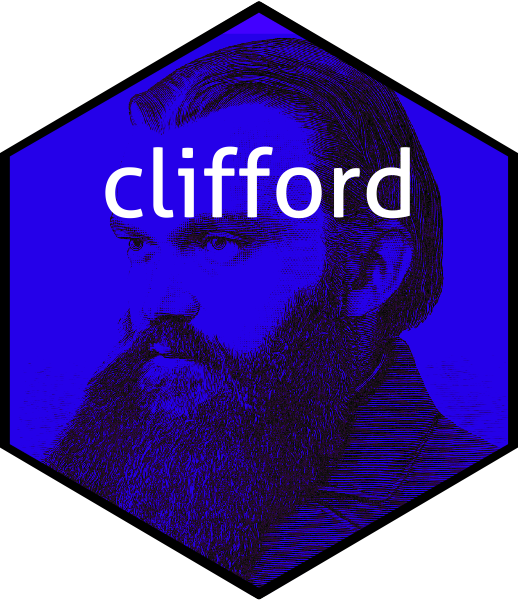
\includegraphics[width=1in]{clifford.png}

\section{Introduction}

Clifford algebras are interesting and instructive mathematical
objects.  The class has a rich structure that has varied applications
to physics.

\subsection{Existing work}

Computational support for working with the Clifford algebras is part
of a number of algebra systems including Sage~\citep{sagemath2019} and
\textit{sympy}~\citep{sympy2017}.  Here I introduce the
\textit{clifford} package, which provides R-centric functionality for
Clifford algebras.  Notation follows~\cite{snygg2010}.


\newcommand{\ei}[1]{\ensuremath{{\bf e}_{#1}}}
\newcommand{\bx}{\ensuremath{{\bf x}}}
\newcommand{\by}{\ensuremath{{\bf y}}}

Considering a vector space of dimension 3, and given a basis
$\ei{1},\ei{2},\ei{3}$, we can consider linear combinations such as

\begin{eqnarray}
\bx = x^1\ei{1} + x^2\ei{2} + x^3\ei{3}\nonumber\\
\by = y^1\ei{1} + y^2\ei{2} + y^3\ei{3}.
\end{eqnarray} 

A Clifford algebra includes a formal product on such sums, defined using the
relations

\begin{eqnarray}\label{square}
\left(\ei{1}\right)^2=
\left(\ei{2}\right)^2=
\left(\ei{3}\right)^2=1\\
\ei{2}\ei{3} + \ei{3}\ei{2} = \label{sumprod}
\ei{1}\ei{3} + \ei{3}\ei{1} = 
\ei{2}\ei{1} + \ei{1}\ei{2} = 0
\end{eqnarray}

This gives:
  
\begin{eqnarray}
\bx\by &=&
\left(x^1\ei{1} + x^2\ei{2} + x^3\ei{3}\right)
\left(y^1\ei{1} + y^2\ei{2} + y^3\ei{3}\right)\nonumber\\
&=& \left(x^1y^1+x^2y^2+x^3y^3\right) +\nonumber\\&&
       \left(x^2y^3-x^3y^2\right)\ei{2}\ei{3} + 
       \left(x^3y^1-x^1y^3\right)\ei{1}\ei{3} + 
       \left(x^1y^2-x^2y^1\right)\ei{1}\ei{2}
\end{eqnarray}
  
Multiplication is associative by design.  \citeauthor{snygg2010} goes
on to consider the algebra spanned by products of
$\ei{1},\ei{2},\ei{3}$ and shows that this is an eight dimensional
space spanned by

\begin{equation}
\left\{
1,\ei{1},\ei{2},\ei{3},\ei{12},\ei{31},\ei{12},\ei{123}
\right\}
\end{equation}

where $\ei{12}=\ei{1}\ei{2}$ and so on.  Thus a general element of
this space would be

\begin{equation}
a^0+
a^1\ei{1} + a^2\ei{2} + a^3\ei{3} +
a^{12}\ei{12} + a^{31}\ei{31} + a^{23}\ei{23} +
a^{123}\ei{123}
\end{equation}

(here the $a$'s are real).  That the space is closed under
multiplication follows from equations~\ref{square} and~\ref{sumprod};
thus, for example,

\begin{equation}
  \ei{1}\ei{3}\ei{1}\ei{2}=
 -\ei{1}\ei{1}\ei{3}\ei{2}=
 -\ei{3}\ei{2}=
  \ei{2}\ei{3}=\ei{23}.
  \end{equation}

(observe how associativity is assumed).

\subsection{Generalization to arbitrary dimensions}

Generalization to higher dimensional vector spaces is easy.  Suppose
we consider a $n$-dimensional vector space spanned by
$\ei{1},\ldots,\ei{n}$.  Then an arbitrary vector in this space will
be $a^1\ei{1}+\cdots+a^n\ei{n}$.  The associated Clifford algebra will
be of dimension $2^n$, spanned by elements like
$\ei{1}\ei{3}\ei{5}=\ei{135}$ and
$\ei{1}\ei{2}\ei{3}\ei{5}=\ei{1235}$.  The defining relations would be

\begin{equation}\label{posdefcliff}
\ei{i}\ei{j}+\ei{j}\ei{i}=2n_{ij}
\end{equation}
where  
\begin{equation}\label{posdefcliff2}
  n_{ij} = \begin{cases}
    1, & i=j\\
    0 &i\neq j
  \end{cases}
\end{equation}



\subsection{Clifford algebra in a pseudo-Euclidean space}

Equations~\ref{posdefcliff} and~\ref{posdefcliff2} defined a
positive-definite inner product on the vector space spanned
by~$\ei{1},\ei{2},\ei{3}$.  This is readily generalized to allow a
more general inner product.  Conventionally we define

\begin{equation}\label{gencliff1}
\ei{i}\ei{j}+\ei{j}\ei{i}=2n_{ij}
\end{equation}
where  
\begin{equation}\label{gencliff2}
  n_{ij} = \begin{cases}
    1, & i=j=1,\ldots,p\\
    -1, & i=j=p+1,\ldots,n\\
    0, &i\neq j
  \end{cases}
\end{equation}

for $1\leqslant p\leqslant n$; usually we also specify $p+q=n$ and
write $\mathbb{R}_{p,q}$ for the $p+q$-dimensional vector space with
inner product given by equation~\ref{gencliff1}.  The Clifford algebra
${\mathcal C}_{p,q}$ (other notations include $Cl(p,q)$) is then the
algebra formed by $\mathbb{R}_{p,q}$ together with formal products of
basis vectors.


Note carefully that the diagonal matrix of the inner product specified
above conventionally has the the positive elements first, followed by
the negative elements.  But in relativity, the metric tensor $\eta$ is
usually written with the negative elements first followed by the
positive elements;

\begin{equation}\eta=
  \begin{bmatrix}
    -1&0&0&0\\
    0&1&0&0\\
    0&0&1&0\\
    0&0&0&1\\
  \end{bmatrix}
\end{equation}


\subsection{Wedge product of the exterior algebra is a special case
  of the geometric product}

If we specify that the quadratic form is identically zero then
equation \ref{gencliff1} becomes

\begin{equation}\label{specwedge}
\ei{i}\ei{j}+\ei{j}\ei{i}=0,\qquad 1\leqslant i,j\leqslant p
\end{equation}

which implies that $\ei{i}\ei{i}=0$.  Geometric products become wedge
products (although linearity means that we may add terms of different
grades, unlike conventional Grassman algebra).

\section{The package in use}

Suppose we want to work with arbitrary Clifford object
$1+2\ei{1}+3\ei{2}+4\ei{2}\ei{3}$.  In R idiom this would be

\begin{Schunk}
\begin{Sinput}
> (x <- clifford(list(numeric(0),1,2,2:3),1:4))
\end{Sinput}
\begin{Soutput}
Element of a Clifford algebra, equal to
+ 1 + 2e_1 + 3e_2 + 4e_23
\end{Soutput}
\end{Schunk}

Function {\tt clifford()} takes a list of terms and a vector of
coefficients.  Addition and subtraction work as expected:

\begin{Schunk}
\begin{Sinput}
> y <- clifford(list(1),2)
> x-y
\end{Sinput}
\begin{Soutput}
Element of a Clifford algebra, equal to
+ 1 + 3e_2 + 4e_23
\end{Soutput}
\end{Schunk}

In the above, see how the $\ei{1}$ term has vanished.  We can
multiply Clifford elements using natural R idiom:

\begin{Schunk}
\begin{Sinput}
> x*x
\end{Sinput}
\begin{Soutput}
Element of a Clifford algebra, equal to
- 2 + 4e_1 + 6e_2 + 8e_23 + 16e_123
\end{Soutput}
\end{Schunk}

(Multiplication that Snygg denotes by juxtaposition is here indicated
with a {\tt *}).  We can consider arbitrarily high dimensional data:

\begin{Schunk}
\begin{Sinput}
> (z <- as.1vector(1:7))
\end{Sinput}
\begin{Soutput}
Element of a Clifford algebra, equal to
+ 1e_1 + 2e_2 + 3e_3 + 4e_4 + 5e_5 + 6e_6 + 7e_7
\end{Soutput}
\begin{Sinput}
> z*x
\end{Sinput}
\begin{Soutput}
Element of a Clifford algebra, equal to
+ 8 + 1e_1 - 10e_2 - 1e_12 + 11e_3 - 6e_13 - 9e_23 + 4e_123 + 4e_4 - 8e_14 -
12e_24 + 16e_234 + 5e_5 - 10e_15 - 15e_25 + 20e_235 + 6e_6 - 12e_16 - 18e_26 +
24e_236 + 7e_7 - 14e_17 - 21e_27 + 28e_237
\end{Soutput}
\end{Schunk}

In the above, we coerce a vector to a Clifford 1-vector.  The package
includes many functions to generate Clifford objects:

\begin{Schunk}
\begin{Sinput}
> rcliff()
\end{Sinput}
\begin{Soutput}
Element of a Clifford algebra, equal to
+ 4 - 2e_4 + 4e_24 + 5e_1234 - 1e_15 + 1e_35 - 3e_45 + 2e_256
\end{Soutput}
\end{Schunk}

The defaults for {\tt rcliff()} specify that the object is a sum of
grade-4 terms but this can be altered:

\begin{Schunk}
\begin{Sinput}
> (x <- rcliff(d=7,g=5,include.fewer=TRUE))
\end{Sinput}
\begin{Soutput}
Element of a Clifford algebra, equal to
+ 4 + 1e_4 - 3e_6 + 3e_12356 + 2e_7 - 1e_23467 + 4e_567 + 5e_3567
\end{Soutput}
\begin{Sinput}
> grades(x)
\end{Sinput}
\begin{Soutput}
A disord object with hash 2d7dd83887de1b90a47d1fef514bb2f733b30b83 and elements
[1] 0 1 1 5 1 5 3 4
(in some order)
\end{Soutput}
\end{Schunk}


\section{Pseudo-Euclidean spaces}

The signature of the metric may be altered.  Starting with the
Euclidean case we have:
    
\begin{Schunk}
\begin{Sinput}
> e1 <- e(1)
> e2 <- e(2)
> e1*e1
\end{Sinput}
\begin{Soutput}
Element of a Clifford algebra, equal to
scalar ( 1 )
\end{Soutput}
\begin{Sinput}
> e2*e2
\end{Sinput}
\begin{Soutput}
Element of a Clifford algebra, equal to
scalar ( 1 )
\end{Soutput}
\end{Schunk}

(function {\tt e(i)} returns $\ei{i}$).  However, if we wish to
consider $n=\begin{bmatrix}1&0\\0&-1\end{bmatrix}$, the package idiom
is to use the {\tt signature()} function:

\begin{Schunk}
\begin{Sinput}
> signature(1,1)  # signature +-
> e1*e1 # as before, returns +1
\end{Sinput}
\begin{Soutput}
Element of a Clifford algebra, equal to
scalar ( 1 )
\end{Soutput}
\begin{Sinput}
> e2*e2 # should return -1
\end{Sinput}
\begin{Soutput}
Element of a Clifford algebra, equal to
scalar ( -1 )
\end{Soutput}
\end{Schunk}

Suppose we wish to use a signature $+++-$, corresponding to the
Minkowski metric in special relativity; this would be indicated in
package idiom by {\tt signature(3,1)}.  Note that the clifford objects
themselves do not store the signature; it is used only by the product
operation {\tt *}.

\begin{Schunk}
\begin{Sinput}
> x <- rcliff(d=4,g=3,include.fewer=TRUE)
> y <- rcliff(d=4,g=3,include.fewer=TRUE)
\end{Sinput}
\end{Schunk}

Then we may multiply these two clifford objects using either the
default positive-definite inner product, or the Minkowski metric:

\begin{Schunk}
\begin{Sinput}
> x*y
\end{Sinput}
\begin{Soutput}
Element of a Clifford algebra, equal to
+ 12 + 12e_1 - 6e_2 + 6e_12 + 7e_3 - 7e_13 + 21e_23 + 13e_123 + 9e_24 + 9e_124
+ 2e_34 + 8e_134 + 19e_234 - 11e_1234
\end{Soutput}
\begin{Sinput}
> signature(3,1)  # switch to signature +++-
> x*y
\end{Sinput}
\begin{Soutput}
Element of a Clifford algebra, equal to
+ 30 + 16e_1 + 2e_12 + 5e_3 - 11e_13 + 21e_23 + 16e_123 - 1e_4 - 18e_14 +
14e_24 + 17e_124 - 2e_34 + 19e_234 - 11e_1234
\end{Soutput}
\end{Schunk}

In the above, see how the products are different using the two inner
products.  

\section{Grassman algebra}

A Grassman algebra corresponds to a Clifford algebra with identically
zero inner product.  Package idiom is to use a zero signature:

\begin{Schunk}
\begin{Sinput}
> signature(0,0)  # specify null inner product
\end{Sinput}
\end{Schunk}
\begin{Schunk}
\begin{Sinput}
> is.zero(e(5)^2)     # should be TRUE
\end{Sinput}
\begin{Soutput}
[1] TRUE
\end{Soutput}
\end{Schunk}

This is a somewhat clunky way of reproducing the functionality of the
{\tt stokes} package.  If we have

\begin{Schunk}
\begin{Sinput}
> x <- clifford(list(1:3, c(2,3,7)), coeffs=3:4)
> y <- clifford(list(1:3, c(1,4,5), c(4,5,6)), coeffs=1:3)
> x %^% y
\end{Sinput}
\begin{Soutput}
Element of a Clifford algebra, equal to
+ 9e_123456 - 8e_123457 - 12e_234567
\end{Soutput}
\end{Schunk}

then the {\tt stokes} idiom for this would be:

\begin{Schunk}
\begin{Sinput}
> (x <- as.kform(rbind(1:3,c(2,3,7)),3:4))
\end{Sinput}
\begin{Soutput}
           val
 2 3 7  =    4
 1 2 3  =    3
\end{Soutput}
\begin{Sinput}
> (y <- as.kform(rbind(1:3,c(1,4,5),4:6),1:3))
\end{Sinput}
\begin{Soutput}
           val
 1 2 3  =    1
 1 4 5  =    2
 4 5 6  =    3
\end{Soutput}
\begin{Sinput}
> x %^% y
\end{Sinput}
\begin{Soutput}
                 val
 1 2 3 4 5 6  =    9
 2 3 4 5 6 7  =  -12
 1 2 3 4 5 7  =   -8
\end{Soutput}
\end{Schunk}


\section{Positive-definite inner product}

Function {\tt signature()} takes an infinite argument to make the
inner product positive-definite:

\begin{Schunk}
\begin{Sinput}
> signature(Inf)
\end{Sinput}
\end{Schunk}

(internally the package sets the signature to
{\tt .Machine\$integer.max}, a near-infinite integer).  With this,
$\ei{i}\ei{i}=+1$ for any $i$:

\begin{Schunk}
\begin{Sinput}
> e(53)^2
\end{Sinput}
\begin{Soutput}
Element of a Clifford algebra, equal to
scalar ( 1 )
\end{Soutput}
\end{Schunk}


\section{Left and right contractions}

\cite{dorst2002} defines the left contraction $A\rfloor B$ and right
contraction $A\lfloor B$ (\cite{chisholm2012} calls these left and
right inner products) as follows:

\begin{eqnarray}
\displaystyle A\rfloor B = \sum_{r,s}\left\langle\left\langle
A\right\rangle_r\left\langle B\right\rangle_s\right\rangle_{s-r}\\
\displaystyle A\lfloor B = \sum_{r,s}\left\langle\left\langle
A\right\rangle_r\left\langle B\right\rangle_s\right\rangle_{r-s}
\end{eqnarray}


Package idiom for these would be {\tt A\%\_|\%B} and {\tt A\%|\_\%B}
---or {\tt lefttick(A,B)} and {\tt righttick(A,B)}---respectively.
Thus:

\begin{Schunk}
\begin{Sinput}
> (A <- rcliff())
\end{Sinput}
\begin{Soutput}
Element of a Clifford algebra, equal to
+ 4 + 2e_2 - 2e_34 + 3e_35 + 5e_235 - 1e_145 + 1e_46 + 4e_156
\end{Soutput}
\begin{Sinput}
> (B <- rcliff())
\end{Sinput}
\begin{Soutput}
Element of a Clifford algebra, equal to
+ 3 - 3e_1 - 1e_13 + 2e_4 + 1e_34 + 3e_135 + 4e_345
\end{Soutput}
\begin{Sinput}
> A %_|% B
\end{Sinput}
\begin{Soutput}
Element of a Clifford algebra, equal to
+ 14 - 21e_1 - 4e_13 + 20e_4 + 4e_34 + 8e_5 + 12e_135 + 16e_345
\end{Soutput}
\begin{Sinput}
> A %|_% B
\end{Sinput}
\begin{Soutput}
Element of a Clifford algebra, equal to
+ 14 + 6e_2 - 4e_3 - 6e_34 + 2e_15 + 9e_35 + 15e_235 + 3e_45 - 3e_145 - 2e_6 +
3e_46 - 12e_56 + 12e_156
\end{Soutput}
\end{Schunk}

One thing to be wary of is the order of operations.  Thus
$\ei{2}\rfloor\ei{12}=-\ei{1}$ (in a positive-definite space) but

\begin{Schunk}
\begin{Sinput}
> e(2) %_|% e(1)*e(2)
\end{Sinput}
\begin{Soutput}
Element of a Clifford algebra, equal to
the zero clifford element (0)
\end{Soutput}
\end{Schunk}

because this is parsed as $(\ei{2}\rfloor\ei{1})\ei{2}=0\ei{2}=0$.  To
evaluate this as intended we need to include brackets:

\begin{Schunk}
\begin{Sinput}
> e(2) %_|% (e(1)*e(2))
\end{Sinput}
\begin{Soutput}
Element of a Clifford algebra, equal to
- 1e_1
\end{Soutput}
\end{Schunk}

although in this case it might be preferable to create the terms directly:

\begin{Schunk}
\begin{Sinput}
> e(2) %_|% e(1:2)
\end{Sinput}
\begin{Soutput}
Element of a Clifford algebra, equal to
- 1e_1
\end{Soutput}
\end{Schunk}


\subsection{Numerical verification of left and right inner product identities}

Chisholm gives a number of identities for these products including

\begin{eqnarray}
  A\rfloor(B\lfloor C) &=& (A\rfloor B)\lfloor C\\
  A\rfloor(B\rfloor C) &=& (A\wedge B)\rfloor C\\
  A\lfloor(B\wedge  C) &=& (A\lfloor B)\lfloor C
\end{eqnarray}

In package idiom:

\begin{Schunk}
\begin{Sinput}
> A <- rcliff();  B <- rcliff();  C <- rcliff()
> A %_|% (B %|_% C) == (A %_|% B) %|_% C
\end{Sinput}
\begin{Soutput}
[1] TRUE
\end{Soutput}
\begin{Sinput}
> A %_|% (B %_|% C) == (A %^%  B) %_|% C
\end{Sinput}
\begin{Soutput}
[1] TRUE
\end{Soutput}
\begin{Sinput}
> A %|_% (B %^%  C) == (A %|_% B) %|_% C
\end{Sinput}
\begin{Soutput}
[1] TRUE
\end{Soutput}
\end{Schunk}
\section{Higher dimensional spaces}

\cite{ablamowicz2012} consider high-dimensional Clifford algebras and
consider the following two elements of the 1024-dimensional Clifford
algebra which we may treat as ${\mathcal C}_{7,3}$ spanned by
$\ei{1},\ldots,\ei{10}$ and perform a calculation which I reproduce
below (although \citeauthor{ablamowicz2012} exploited Bott
periodicity, a feature not considered here).

Firstly we change the default print method slightly:

\begin{Schunk}
\begin{Sinput}
> options("basissep" = ",")
\end{Sinput}
\end{Schunk}

(this separates the subscripts of the basis vectors with a comma,
which is useful for clarity if $n>9$).  We then define clifford
elements $x,y$:

\begin{Schunk}
\begin{Sinput}
> (x <- clifford(list(1:3,c(1,5,7,8,10)),c(4,-10)) + 2)
\end{Sinput}
\begin{Soutput}
Element of a Clifford algebra, equal to
+ 2 + 4e_1,2,3 - 10e_1,5,7,8,10
\end{Soutput}
\begin{Sinput}
> (y <- clifford(list(c(1,2,3,7),c(1,5,6,8),c(1,4,6,7)),c(4,1,-3)) - 1)
\end{Sinput}
\begin{Soutput}
Element of a Clifford algebra, equal to
- 1 + 4e_1,2,3,7 - 3e_1,4,6,7 + 1e_1,5,6,8
\end{Soutput}
\end{Schunk}

Their geometric product is given in the package as

\begin{Schunk}
\begin{Sinput}
> signature(7)
> x*y
\end{Sinput}
\begin{Soutput}
Element of a Clifford algebra, equal to
- 2 - 4e_1,2,3 - 16e_7 + 8e_1,2,3,7 - 6e_1,4,6,7 - 12e_2,3,4,6,7 + 2e_1,5,6,8 +
4e_2,3,5,6,8 - 40e_2,3,5,8,10 - 30e_4,5,6,8,10 + 10e_1,5,7,8,10
\end{Soutput}
\end{Schunk}

in agreement with \cite{ablamowicz2012}, although the terms appear in
a different order.

\section{Conclusions and further work}

The {\tt clifford} package furnishes a consistent and documented suite
of reasonably efficient {\tt R}-centric functionality.  Further
work might include closer integration with the {\tt stokes}
package~\citep{hankin2019}.


 
\bibliographystyle{apalike}
% -*- mode: noweb; noweb-default-code-mode: R-mode; -*-


\documentclass{article}

\usepackage{arxiv}

\usepackage[utf8]{inputenc} % allow utf-8 input
\usepackage[T1]{fontenc}    % use 8-bit T1 fonts
\usepackage{hyperref}       % hyperlinks
\usepackage{url}            % simple URL typesetting
\usepackage{booktabs}       % professional-quality tables
\usepackage{amsfonts}       % blackboard math symbols
\usepackage{amssymb}        % needed for \leqslant
\usepackage{amsmath}        % needed for cases
\usepackage{nicefrac}       % compact symbols for 1/2, etc.
\usepackage{microtype}      % microtypography
\usepackage{lipsum}		% Can be removed after putting your text content
\usepackage{graphicx}
\usepackage{natbib}
\usepackage{doi}



\title{Clifford algebra in R}

%\date{September 9, 1985}	% Here you can change the date presented in the paper title
%\date{} 					% Or removing it

\author{ \href{https://orcid.org/0000-0001-5982-0415}{\includegraphics[width=0.03\textwidth]{orcid.pdf}\hspace{1mm}Robin K. S.~Hankin}\thanks{\href{https://academics.aut.ac.nz/robin.hankin}{work};  
\href{https://www.youtube.com/watch?v=JzCX3FqDIOc&list=PL9_n3Tqzq9iWtgD8POJFdnVUCZ_zw6OiB&ab_channel=TrinTragulaGeneralRelativity}{play}} \\
 Auckland University of Technology\\
	\texttt{hankin.robin@gmail.com} \\
}

% Uncomment to remove the date
%\date{}

% Uncomment to override  the `A preprint' in the header
%\renewcommand{\headeright}{Technical Report}
%\renewcommand{\undertitle}{Technical Report}
\renewcommand{\shorttitle}{The \textit{clifford} package}

%%% Add PDF metadata to help others organize their library
%%% Once the PDF is generated, you can check the metadata with
%%% $ pdfinfo template.pdf
\hypersetup{
pdftitle={Clifford algebra in R},
pdfsubject={q-bio.NC, q-bio.QM},
pdfauthor={Robin K. S.~Hankin},
pdfkeywords={Clifford algebra}
}

\usepackage{Sweave}
\begin{document}
\maketitle

\begin{abstract}
Here I present the {\tt clifford} package for working with Clifford
algebras in the R programming language.  The algebra is described and
package idiom is given.
\end{abstract}


% keywords can be removed
\keywords{Clifford algebra}



\hfill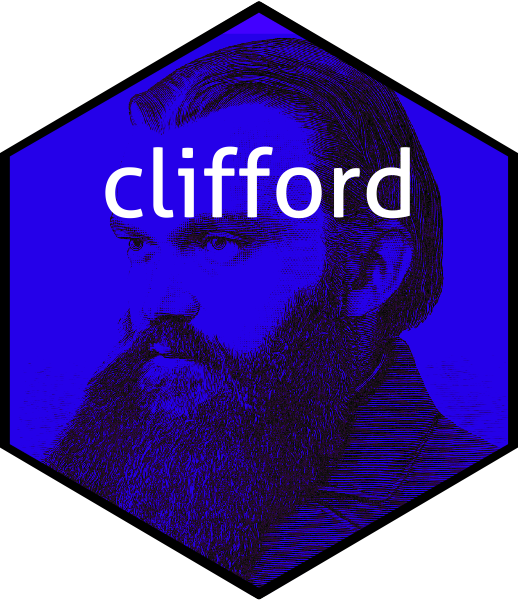
\includegraphics[width=1in]{clifford.png}

\section{Introduction}

Clifford algebras are interesting and instructive mathematical
objects.  The class has a rich structure that has varied applications
to physics.

\subsection{Existing work}

Computational support for working with the Clifford algebras is part
of a number of algebra systems including Sage~\citep{sagemath2019} and
\textit{sympy}~\citep{sympy2017}.  Here I introduce the
\textit{clifford} package, which provides R-centric functionality for
Clifford algebras.  Notation follows~\cite{snygg2010}.


\newcommand{\ei}[1]{\ensuremath{{\bf e}_{#1}}}
\newcommand{\bx}{\ensuremath{{\bf x}}}
\newcommand{\by}{\ensuremath{{\bf y}}}

Considering a vector space of dimension 3, and given a basis
$\ei{1},\ei{2},\ei{3}$, we can consider linear combinations such as

\begin{eqnarray}
\bx = x^1\ei{1} + x^2\ei{2} + x^3\ei{3}\nonumber\\
\by = y^1\ei{1} + y^2\ei{2} + y^3\ei{3}.
\end{eqnarray} 

A Clifford algebra includes a formal product on such sums, defined using the
relations

\begin{eqnarray}\label{square}
\left(\ei{1}\right)^2=
\left(\ei{2}\right)^2=
\left(\ei{3}\right)^2=1\\
\ei{2}\ei{3} + \ei{3}\ei{2} = \label{sumprod}
\ei{1}\ei{3} + \ei{3}\ei{1} = 
\ei{2}\ei{1} + \ei{1}\ei{2} = 0
\end{eqnarray}

This gives:
  
\begin{eqnarray}
\bx\by &=&
\left(x^1\ei{1} + x^2\ei{2} + x^3\ei{3}\right)
\left(y^1\ei{1} + y^2\ei{2} + y^3\ei{3}\right)\nonumber\\
&=& \left(x^1y^1+x^2y^2+x^3y^3\right) +\nonumber\\&&
       \left(x^2y^3-x^3y^2\right)\ei{2}\ei{3} + 
       \left(x^3y^1-x^1y^3\right)\ei{1}\ei{3} + 
       \left(x^1y^2-x^2y^1\right)\ei{1}\ei{2}
\end{eqnarray}
  
Multiplication is associative by design.  \citeauthor{snygg2010} goes
on to consider the algebra spanned by products of
$\ei{1},\ei{2},\ei{3}$ and shows that this is an eight dimensional
space spanned by

\begin{equation}
\left\{
1,\ei{1},\ei{2},\ei{3},\ei{12},\ei{31},\ei{12},\ei{123}
\right\}
\end{equation}

where $\ei{12}=\ei{1}\ei{2}$ and so on.  Thus a general element of
this space would be

\begin{equation}
a^0+
a^1\ei{1} + a^2\ei{2} + a^3\ei{3} +
a^{12}\ei{12} + a^{31}\ei{31} + a^{23}\ei{23} +
a^{123}\ei{123}
\end{equation}

(here the $a$'s are real).  That the space is closed under
multiplication follows from equations~\ref{square} and~\ref{sumprod};
thus, for example,

\begin{equation}
  \ei{1}\ei{3}\ei{1}\ei{2}=
 -\ei{1}\ei{1}\ei{3}\ei{2}=
 -\ei{3}\ei{2}=
  \ei{2}\ei{3}=\ei{23}.
  \end{equation}

(observe how associativity is assumed).

\subsection{Generalization to arbitrary dimensions}

Generalization to higher dimensional vector spaces is easy.  Suppose
we consider a $n$-dimensional vector space spanned by
$\ei{1},\ldots,\ei{n}$.  Then an arbitrary vector in this space will
be $a^1\ei{1}+\cdots+a^n\ei{n}$.  The associated Clifford algebra will
be of dimension $2^n$, spanned by elements like
$\ei{1}\ei{3}\ei{5}=\ei{135}$ and
$\ei{1}\ei{2}\ei{3}\ei{5}=\ei{1235}$.  The defining relations would be

\begin{equation}\label{posdefcliff}
\ei{i}\ei{j}+\ei{j}\ei{i}=2n_{ij}
\end{equation}
where  
\begin{equation}\label{posdefcliff2}
  n_{ij} = \begin{cases}
    1, & i=j\\
    0 &i\neq j
  \end{cases}
\end{equation}



\subsection{Clifford algebra in a pseudo-Euclidean space}

Equations~\ref{posdefcliff} and~\ref{posdefcliff2} defined a
positive-definite inner product on the vector space spanned
by~$\ei{1},\ei{2},\ei{3}$.  This is readily generalized to allow a
more general inner product.  Conventionally we define

\begin{equation}\label{gencliff1}
\ei{i}\ei{j}+\ei{j}\ei{i}=2n_{ij}
\end{equation}
where  
\begin{equation}\label{gencliff2}
  n_{ij} = \begin{cases}
    1, & i=j=1,\ldots,p\\
    -1, & i=j=p+1,\ldots,n\\
    0, &i\neq j
  \end{cases}
\end{equation}

for $1\leqslant p\leqslant n$; usually we also specify $p+q=n$ and
write $\mathbb{R}_{p,q}$ for the $p+q$-dimensional vector space with
inner product given by equation~\ref{gencliff1}.  The Clifford algebra
${\mathcal C}_{p,q}$ (other notations include $Cl(p,q)$) is then the
algebra formed by $\mathbb{R}_{p,q}$ together with formal products of
basis vectors.


Note carefully that the diagonal matrix of the inner product specified
above conventionally has the the positive elements first, followed by
the negative elements.  But in relativity, the metric tensor $\eta$ is
usually written with the negative elements first followed by the
positive elements;

\begin{equation}\eta=
  \begin{bmatrix}
    -1&0&0&0\\
    0&1&0&0\\
    0&0&1&0\\
    0&0&0&1\\
  \end{bmatrix}
\end{equation}


\subsection{Wedge product of the exterior algebra is a special case
  of the geometric product}

If we specify that the quadratic form is identically zero then
equation \ref{gencliff1} becomes

\begin{equation}\label{specwedge}
\ei{i}\ei{j}+\ei{j}\ei{i}=0,\qquad 1\leqslant i,j\leqslant p
\end{equation}

which implies that $\ei{i}\ei{i}=0$.  Geometric products become wedge
products (although linearity means that we may add terms of different
grades, unlike conventional Grassman algebra).

\section{The package in use}

Suppose we want to work with arbitrary Clifford object
$1+2\ei{1}+3\ei{2}+4\ei{2}\ei{3}$.  In R idiom this would be

\begin{Schunk}
\begin{Sinput}
> (x <- clifford(list(numeric(0),1,2,2:3),1:4))
\end{Sinput}
\begin{Soutput}
Element of a Clifford algebra, equal to
+ 1 + 2e_1 + 3e_2 + 4e_23
\end{Soutput}
\end{Schunk}

Function {\tt clifford()} takes a list of terms and a vector of
coefficients.  Addition and subtraction work as expected:

\begin{Schunk}
\begin{Sinput}
> y <- clifford(list(1),2)
> x-y
\end{Sinput}
\begin{Soutput}
Element of a Clifford algebra, equal to
+ 1 + 3e_2 + 4e_23
\end{Soutput}
\end{Schunk}

In the above, see how the $\ei{1}$ term has vanished.  We can
multiply Clifford elements using natural R idiom:

\begin{Schunk}
\begin{Sinput}
> x*x
\end{Sinput}
\begin{Soutput}
Element of a Clifford algebra, equal to
- 2 + 4e_1 + 6e_2 + 8e_23 + 16e_123
\end{Soutput}
\end{Schunk}

(Multiplication that Snygg denotes by juxtaposition is here indicated
with a {\tt *}).  We can consider arbitrarily high dimensional data:

\begin{Schunk}
\begin{Sinput}
> (z <- as.1vector(1:7))
\end{Sinput}
\begin{Soutput}
Element of a Clifford algebra, equal to
+ 1e_1 + 2e_2 + 3e_3 + 4e_4 + 5e_5 + 6e_6 + 7e_7
\end{Soutput}
\begin{Sinput}
> z*x
\end{Sinput}
\begin{Soutput}
Element of a Clifford algebra, equal to
+ 8 + 1e_1 - 10e_2 - 1e_12 + 11e_3 - 6e_13 - 9e_23 + 4e_123 + 4e_4 - 8e_14 -
12e_24 + 16e_234 + 5e_5 - 10e_15 - 15e_25 + 20e_235 + 6e_6 - 12e_16 - 18e_26 +
24e_236 + 7e_7 - 14e_17 - 21e_27 + 28e_237
\end{Soutput}
\end{Schunk}

In the above, we coerce a vector to a Clifford 1-vector.  The package
includes many functions to generate Clifford objects:

\begin{Schunk}
\begin{Sinput}
> rcliff()
\end{Sinput}
\begin{Soutput}
Element of a Clifford algebra, equal to
+ 4 - 2e_4 + 4e_24 + 5e_1234 - 1e_15 + 1e_35 - 3e_45 + 2e_256
\end{Soutput}
\end{Schunk}

The defaults for {\tt rcliff()} specify that the object is a sum of
grade-4 terms but this can be altered:

\begin{Schunk}
\begin{Sinput}
> (x <- rcliff(d=7,g=5,include.fewer=TRUE))
\end{Sinput}
\begin{Soutput}
Element of a Clifford algebra, equal to
+ 4 + 1e_4 - 3e_6 + 3e_12356 + 2e_7 - 1e_23467 + 4e_567 + 5e_3567
\end{Soutput}
\begin{Sinput}
> grades(x)
\end{Sinput}
\begin{Soutput}
A disord object with hash 2d7dd83887de1b90a47d1fef514bb2f733b30b83 and elements
[1] 0 1 1 5 1 5 3 4
(in some order)
\end{Soutput}
\end{Schunk}


\section{Pseudo-Euclidean spaces}

The signature of the metric may be altered.  Starting with the
Euclidean case we have:
    
\begin{Schunk}
\begin{Sinput}
> e1 <- e(1)
> e2 <- e(2)
> e1*e1
\end{Sinput}
\begin{Soutput}
Element of a Clifford algebra, equal to
scalar ( 1 )
\end{Soutput}
\begin{Sinput}
> e2*e2
\end{Sinput}
\begin{Soutput}
Element of a Clifford algebra, equal to
scalar ( 1 )
\end{Soutput}
\end{Schunk}

(function {\tt e(i)} returns $\ei{i}$).  However, if we wish to
consider $n=\begin{bmatrix}1&0\\0&-1\end{bmatrix}$, the package idiom
is to use the {\tt signature()} function:

\begin{Schunk}
\begin{Sinput}
> signature(1,1)  # signature +-
> e1*e1 # as before, returns +1
\end{Sinput}
\begin{Soutput}
Element of a Clifford algebra, equal to
scalar ( 1 )
\end{Soutput}
\begin{Sinput}
> e2*e2 # should return -1
\end{Sinput}
\begin{Soutput}
Element of a Clifford algebra, equal to
scalar ( -1 )
\end{Soutput}
\end{Schunk}

Suppose we wish to use a signature $+++-$, corresponding to the
Minkowski metric in special relativity; this would be indicated in
package idiom by {\tt signature(3,1)}.  Note that the clifford objects
themselves do not store the signature; it is used only by the product
operation {\tt *}.

\begin{Schunk}
\begin{Sinput}
> x <- rcliff(d=4,g=3,include.fewer=TRUE)
> y <- rcliff(d=4,g=3,include.fewer=TRUE)
\end{Sinput}
\end{Schunk}

Then we may multiply these two clifford objects using either the
default positive-definite inner product, or the Minkowski metric:

\begin{Schunk}
\begin{Sinput}
> x*y
\end{Sinput}
\begin{Soutput}
Element of a Clifford algebra, equal to
+ 12 + 12e_1 - 6e_2 + 6e_12 + 7e_3 - 7e_13 + 21e_23 + 13e_123 + 9e_24 + 9e_124
+ 2e_34 + 8e_134 + 19e_234 - 11e_1234
\end{Soutput}
\begin{Sinput}
> signature(3,1)  # switch to signature +++-
> x*y
\end{Sinput}
\begin{Soutput}
Element of a Clifford algebra, equal to
+ 30 + 16e_1 + 2e_12 + 5e_3 - 11e_13 + 21e_23 + 16e_123 - 1e_4 - 18e_14 +
14e_24 + 17e_124 - 2e_34 + 19e_234 - 11e_1234
\end{Soutput}
\end{Schunk}

In the above, see how the products are different using the two inner
products.  

\section{Grassman algebra}

A Grassman algebra corresponds to a Clifford algebra with identically
zero inner product.  Package idiom is to use a zero signature:

\begin{Schunk}
\begin{Sinput}
> signature(0,0)  # specify null inner product
\end{Sinput}
\end{Schunk}
\begin{Schunk}
\begin{Sinput}
> is.zero(e(5)^2)     # should be TRUE
\end{Sinput}
\begin{Soutput}
[1] TRUE
\end{Soutput}
\end{Schunk}

This is a somewhat clunky way of reproducing the functionality of the
{\tt stokes} package.  If we have

\begin{Schunk}
\begin{Sinput}
> x <- clifford(list(1:3, c(2,3,7)), coeffs=3:4)
> y <- clifford(list(1:3, c(1,4,5), c(4,5,6)), coeffs=1:3)
> x %^% y
\end{Sinput}
\begin{Soutput}
Element of a Clifford algebra, equal to
+ 9e_123456 - 8e_123457 - 12e_234567
\end{Soutput}
\end{Schunk}

then the {\tt stokes} idiom for this would be:

\begin{Schunk}
\begin{Sinput}
> (x <- as.kform(rbind(1:3,c(2,3,7)),3:4))
\end{Sinput}
\begin{Soutput}
           val
 2 3 7  =    4
 1 2 3  =    3
\end{Soutput}
\begin{Sinput}
> (y <- as.kform(rbind(1:3,c(1,4,5),4:6),1:3))
\end{Sinput}
\begin{Soutput}
           val
 1 2 3  =    1
 1 4 5  =    2
 4 5 6  =    3
\end{Soutput}
\begin{Sinput}
> x %^% y
\end{Sinput}
\begin{Soutput}
                 val
 1 2 3 4 5 6  =    9
 2 3 4 5 6 7  =  -12
 1 2 3 4 5 7  =   -8
\end{Soutput}
\end{Schunk}


\section{Positive-definite inner product}

Function {\tt signature()} takes an infinite argument to make the
inner product positive-definite:

\begin{Schunk}
\begin{Sinput}
> signature(Inf)
\end{Sinput}
\end{Schunk}

(internally the package sets the signature to
{\tt .Machine\$integer.max}, a near-infinite integer).  With this,
$\ei{i}\ei{i}=+1$ for any $i$:

\begin{Schunk}
\begin{Sinput}
> e(53)^2
\end{Sinput}
\begin{Soutput}
Element of a Clifford algebra, equal to
scalar ( 1 )
\end{Soutput}
\end{Schunk}


\section{Left and right contractions}

\cite{dorst2002} defines the left contraction $A\rfloor B$ and right
contraction $A\lfloor B$ (\cite{chisholm2012} calls these left and
right inner products) as follows:

\begin{eqnarray}
\displaystyle A\rfloor B = \sum_{r,s}\left\langle\left\langle
A\right\rangle_r\left\langle B\right\rangle_s\right\rangle_{s-r}\\
\displaystyle A\lfloor B = \sum_{r,s}\left\langle\left\langle
A\right\rangle_r\left\langle B\right\rangle_s\right\rangle_{r-s}
\end{eqnarray}


Package idiom for these would be {\tt A\%\_|\%B} and {\tt A\%|\_\%B}
---or {\tt lefttick(A,B)} and {\tt righttick(A,B)}---respectively.
Thus:

\begin{Schunk}
\begin{Sinput}
> (A <- rcliff())
\end{Sinput}
\begin{Soutput}
Element of a Clifford algebra, equal to
+ 4 + 2e_2 - 2e_34 + 3e_35 + 5e_235 - 1e_145 + 1e_46 + 4e_156
\end{Soutput}
\begin{Sinput}
> (B <- rcliff())
\end{Sinput}
\begin{Soutput}
Element of a Clifford algebra, equal to
+ 3 - 3e_1 - 1e_13 + 2e_4 + 1e_34 + 3e_135 + 4e_345
\end{Soutput}
\begin{Sinput}
> A %_|% B
\end{Sinput}
\begin{Soutput}
Element of a Clifford algebra, equal to
+ 14 - 21e_1 - 4e_13 + 20e_4 + 4e_34 + 8e_5 + 12e_135 + 16e_345
\end{Soutput}
\begin{Sinput}
> A %|_% B
\end{Sinput}
\begin{Soutput}
Element of a Clifford algebra, equal to
+ 14 + 6e_2 - 4e_3 - 6e_34 + 2e_15 + 9e_35 + 15e_235 + 3e_45 - 3e_145 - 2e_6 +
3e_46 - 12e_56 + 12e_156
\end{Soutput}
\end{Schunk}

One thing to be wary of is the order of operations.  Thus
$\ei{2}\rfloor\ei{12}=-\ei{1}$ (in a positive-definite space) but

\begin{Schunk}
\begin{Sinput}
> e(2) %_|% e(1)*e(2)
\end{Sinput}
\begin{Soutput}
Element of a Clifford algebra, equal to
the zero clifford element (0)
\end{Soutput}
\end{Schunk}

because this is parsed as $(\ei{2}\rfloor\ei{1})\ei{2}=0\ei{2}=0$.  To
evaluate this as intended we need to include brackets:

\begin{Schunk}
\begin{Sinput}
> e(2) %_|% (e(1)*e(2))
\end{Sinput}
\begin{Soutput}
Element of a Clifford algebra, equal to
- 1e_1
\end{Soutput}
\end{Schunk}

although in this case it might be preferable to create the terms directly:

\begin{Schunk}
\begin{Sinput}
> e(2) %_|% e(1:2)
\end{Sinput}
\begin{Soutput}
Element of a Clifford algebra, equal to
- 1e_1
\end{Soutput}
\end{Schunk}


\subsection{Numerical verification of left and right inner product identities}

Chisholm gives a number of identities for these products including

\begin{eqnarray}
  A\rfloor(B\lfloor C) &=& (A\rfloor B)\lfloor C\\
  A\rfloor(B\rfloor C) &=& (A\wedge B)\rfloor C\\
  A\lfloor(B\wedge  C) &=& (A\lfloor B)\lfloor C
\end{eqnarray}

In package idiom:

\begin{Schunk}
\begin{Sinput}
> A <- rcliff();  B <- rcliff();  C <- rcliff()
> A %_|% (B %|_% C) == (A %_|% B) %|_% C
\end{Sinput}
\begin{Soutput}
[1] TRUE
\end{Soutput}
\begin{Sinput}
> A %_|% (B %_|% C) == (A %^%  B) %_|% C
\end{Sinput}
\begin{Soutput}
[1] TRUE
\end{Soutput}
\begin{Sinput}
> A %|_% (B %^%  C) == (A %|_% B) %|_% C
\end{Sinput}
\begin{Soutput}
[1] TRUE
\end{Soutput}
\end{Schunk}
\section{Higher dimensional spaces}

\cite{ablamowicz2012} consider high-dimensional Clifford algebras and
consider the following two elements of the 1024-dimensional Clifford
algebra which we may treat as ${\mathcal C}_{7,3}$ spanned by
$\ei{1},\ldots,\ei{10}$ and perform a calculation which I reproduce
below (although \citeauthor{ablamowicz2012} exploited Bott
periodicity, a feature not considered here).

Firstly we change the default print method slightly:

\begin{Schunk}
\begin{Sinput}
> options("basissep" = ",")
\end{Sinput}
\end{Schunk}

(this separates the subscripts of the basis vectors with a comma,
which is useful for clarity if $n>9$).  We then define clifford
elements $x,y$:

\begin{Schunk}
\begin{Sinput}
> (x <- clifford(list(1:3,c(1,5,7,8,10)),c(4,-10)) + 2)
\end{Sinput}
\begin{Soutput}
Element of a Clifford algebra, equal to
+ 2 + 4e_1,2,3 - 10e_1,5,7,8,10
\end{Soutput}
\begin{Sinput}
> (y <- clifford(list(c(1,2,3,7),c(1,5,6,8),c(1,4,6,7)),c(4,1,-3)) - 1)
\end{Sinput}
\begin{Soutput}
Element of a Clifford algebra, equal to
- 1 + 4e_1,2,3,7 - 3e_1,4,6,7 + 1e_1,5,6,8
\end{Soutput}
\end{Schunk}

Their geometric product is given in the package as

\begin{Schunk}
\begin{Sinput}
> signature(7)
> x*y
\end{Sinput}
\begin{Soutput}
Element of a Clifford algebra, equal to
- 2 - 4e_1,2,3 - 16e_7 + 8e_1,2,3,7 - 6e_1,4,6,7 - 12e_2,3,4,6,7 + 2e_1,5,6,8 +
4e_2,3,5,6,8 - 40e_2,3,5,8,10 - 30e_4,5,6,8,10 + 10e_1,5,7,8,10
\end{Soutput}
\end{Schunk}

in agreement with \cite{ablamowicz2012}, although the terms appear in
a different order.

\section{Conclusions and further work}

The {\tt clifford} package furnishes a consistent and documented suite
of reasonably efficient {\tt R}-centric functionality.  Further
work might include closer integration with the {\tt stokes}
package~\citep{hankin2019}.


 
\bibliographystyle{apalike}
\input{clifford_arxiv.bbl}

\end{document}



\end{document}



\end{document}



\end{document}

